% Template for ICIP-2019 paper; to be used with:
%          spconf.sty  - ICASSP/ICIP LaTeX style file, and
%          IEEEbib.bst - IEEE bibliography style file.
% --------------------------------------------------------------------------
\documentclass{article}
\usepackage{spconf,amsmath,graphicx}

% Example definitions.
% --------------------
\def\x{{\mathbf x}}
\def\L{{\cal L}}

% Title.
% ------
\title{AUTHOR GUIDELINES FOR ICIP 2019 PROCEEDINGS MANUSCRIPTS}
%
% Single address.
% ---------------
\name{Author(s) Name(s)\thanks{Thanks to XYZ agency for funding.}}
\address{Author Affiliation(s)}
%
% For example:
% ------------
%\address{School\\
%	Department\\
%	Address}
%
% Two addresses (uncomment and modify for two-address case).
% ----------------------------------------------------------
%\twoauthors
%  {A. Author-one, B. Author-two\sthanks{Thanks to XYZ agency for funding.}}
%	{School A-B\\
%	Department A-B\\
%	Address A-B}
%  {C. Author-three, D. Author-four\sthanks{The fourth author performed the work
%	while at ...}}
%	{School C-D\\
%	Department C-D\\
%	Address C-D}
%
\begin{document}
%\ninept
%
\maketitle
%
\begin{abstract}
  Producing a high quality image which represents the real world as close as possible is a difficult task. 
  Cameras are limited in their capability to capture a realistic image. 
  One of such limitations is obvious when we try to make a photograph of a scene with very high differences between light and dark areas. 
  In this paper, we will discuss a solution to this limitation - High Dynamic Range image processing. 
  We will explain what does camera, in this context, struggle with and why. 
  Then we will take a look at all the needed components to capture a High Dynamic Range (HDR) image, and how does it look like.
% The abstract should appear at the top of the left-hand column of text, about
% 0.5 inch (12 mm) below the title area and no more than 3.125 inches (80 mm) in
% length.  Leave a 0.5 inch (12 mm) space between the end of the abstract and the
% beginning of the main text.  The abstract should contain about 100 to 150
% words, and should be identical to the abstract text submitted electronically
% along with the paper cover sheet.  All manuscripts must be in English, printed
% in black ink.
\end{abstract}
%
\begin{keywords}
One, two, three, four, five
\end{keywords}
%
\section{Introduction}
\label{sec:intro}
It is not easy to capture a very realistic image. Camera is limited by the currently existing technology and it loses some information when capturing some real life scenes. 
Many problems exist, but our focus in this paper is dynamic range. Capturing a scene with very large differences between dark and light areas in a scene is not a simple task. 
In order to do this, we must find a way to expand the limits of the current technology using clever workarounds and methods.
That in first place includes combining many existing technologies, like computer processing, in such a way that they all work towards the same goal and fill in the gaps of each other. % TODO - improve the introduction. Ich bin sicher jeder kann da was gutes sagen :D

% These guidelines include complete descriptions of the fonts, spacing, and
% related information for producing your proceedings manuscripts. Please follow
% them and if you have any questions, direct them to Conference Management
% Services, Inc.: Phone +1-979-846-6800 or email
% to \\\texttt{icip2019@cmsworkshops.com}.

\section{Dynamic Range} % TODO Johannes bitte schreib hier dein Teil

\subsection{General Definition}
Dynamic Range 

\subsection{High Dynamic Range (HDR)}

\subsection{When should you use HDR}

\subsection{Camera and Dynamic Range}
In order to better understand why is camera not capable of taking a high dynamic range image, we will briefly explain how does a camera work. 
The main component we are interested in is the camera's sensor, built from many pixels.
The photons travel through the camera lens and land onto the sensor. 
Sensor absorbs the photons and interprets them as an electrical signal.
Without going into much detail, pixels in sensors have a certain capacity. Any pixel which reaches this full capacity is going to be interpreted as pure white color in the final image.
\begin{figure}[H]
    \centering
    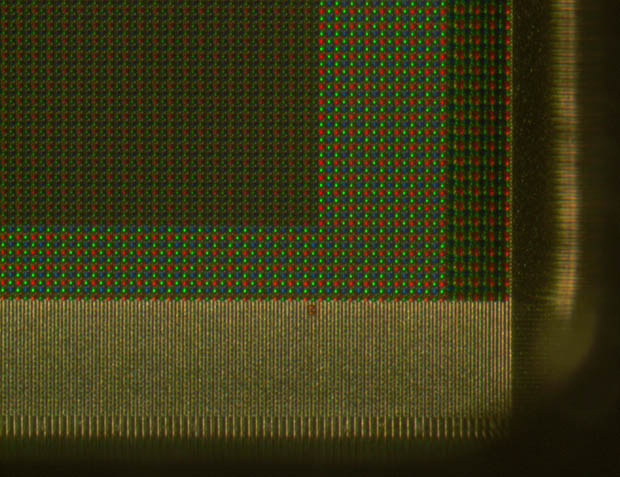
\includegraphics[width = 1.0\linewidth]{images/cmosmicrograph-2.jpg}
    \caption{CMOS Sensor under a Microscope \cite{sensor:Array}}
    \label{fig:sensorArray}
\end{figure}

But, apart from the signal received by absorbing photons, there is some noise the sensor produces.
That means that any pixel which produces signal weaker than the noise of the sensor is not going to give us any meaningful information.
So trying to capture dark part of scene and letting in too many photons in camera leads us to the risk of reaching full
capacity on too many pixels - which in end leads to information loss. 
On the other hand, if we try to prevent that, we may not have enough signal in pixels corresponding to the
darker parts of the scene - which, again, leads to loss of information. 
More often than not the scene we are trying to capture has wider range in lightness than what we have at our disposal.
We are simply forced to "sacrifice" shadows or highlights and sometimes even both.
\begin{figure}[H]
    \centering
    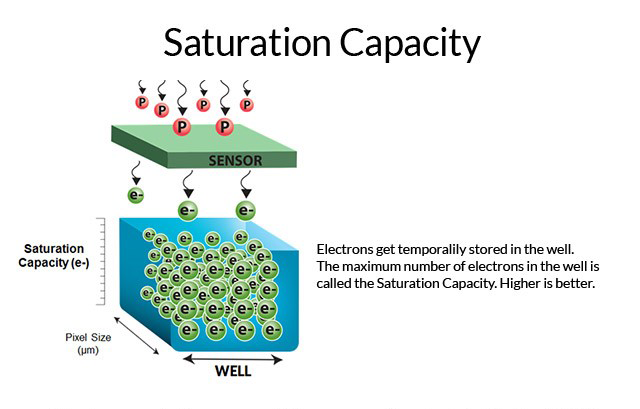
\includegraphics[width = 1.0\linewidth]{images/saturation-capacity-large.png}
    \caption{Illustration of Sensor Pixel Saturation \cite{sensor:Saturation}}
    \label{fig:sensorSaturation}
\end{figure}

\subsection{Image Export and Format}
Electrical signal will be amplified and passed to Analog to Digital converter, which converts the signal into numbers.
Each pixel in an image has three values, one for each color - red, green and blue. 

These numbers then get stored into an image file using one of many image formats. 
One such format is the very known JPEG, which stores 8 bits per color, values range from 0-255.
Another format, or better format category, is the RAW format. This format is capable of storing much more information, 12-14 bits per color. JPEG and similar formats are another point where we can loose information.
It is worth noting that JPEG and similar formats also produce much smaller file sizes and more often than not perform some compression.
Raw formats, on the other hand, have no compression applied and store metadata alongside the color information,
like camera settings at the moment of image capture, camera model, manufacturer etc.

\section{HDR Image Processing}
\subsection{Preparation}
Creating an HDR Image is not a simple task. It involves many steps which are executed either manually, or automatically depending on the use case. 
If camera performs HDR Image Processing at the time of capture, it has all the necessary information, 
can capture all the exposures it needs and perform the HDR Image Processing right away.

However, if we want to capture an HDR Image using any camera, then we must perform these operations ourselves.
Some of the most important steps are:
\begin{itemize}
    \item Image Bracketing - Taking multiple exposures to capture all parts of the scene clearly
    \item Image Alignment - Correcting fine movement introduced in the image bracketing
    \item Camera Response Function - Calculating the light intensity mapping of the camera
    \item Image Combining - Combining all the gathered images into one HDR Image
    \item Tone Mapping - Converting the color values into values compatible with displays
\end{itemize}

\subsection{Image Bracketing}
Image Bracketing is a procedure of taking multiple images with different exposures. 
The point of doing this, is to cover as much of the light spectrum as possible. We try to capture information in the darkest shadows
as well as in the lightest highlights and everything in between.
That way, we go around the camera's limitation in regards to dynamic range. 

Generally, capturing more exposures is better. This depends on the actual scene and how big is the actual difference between the darkest and lightest parts of the scene. It is to be taken as a rule of thumb, and not a hard fact.
Sometimes even two images are enough, but other times many more are needed. 

To successfully perform this task, we start taking exposures where we capture one side of the spectrum, e.g. the light area in the scene.
We should also try to prevent any movement we can. 
It is best done using a tripod and making our camera stationary, instead of holding it in our hands.
Then, we change the camera settings so that we increment the exposure value. 
In other words, we capture a brighter version of the same image by, for example, making exposure time longer.

\begin{figure}[h!]
    \centering
    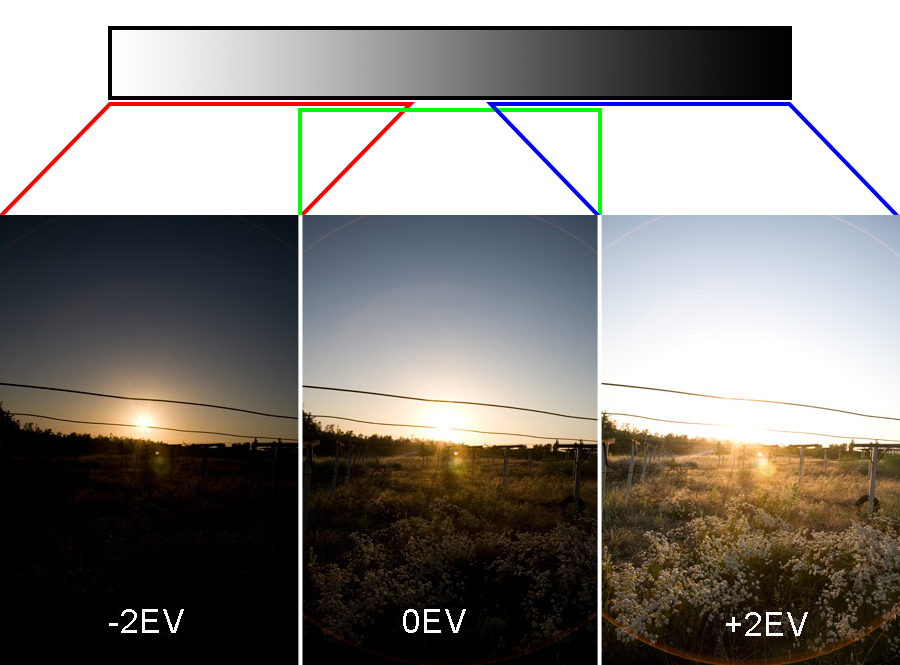
\includegraphics[width = 1.0\linewidth]{images/spectrum3.jpg}
    \caption{Image Bracketing Example \cite{bracketing:Example}}
    \label{fig:imageBracketing}
\end{figure}

We repeat this procedure until we reach the other side of the spectrum.
By doing this, we will capture information in every part of our scene and nothing gets lost.
That means, there is no part of our images which is not clearly visible at least in one of the captured exposures.

\subsection{Image Alignment}
\subsection{Camera Response Function}
\subsection{Image Combining}
\subsection{Tone Mapping}

\section{Possible Problems with HDR Images}
\subsection{Ghosting}
\subsection{Flattening}
\subsection{Halos}


% \section{Formatting your paper}
% \label{sec:format}

% All printed material, including text, illustrations, and charts, must be kept
% within a print area of 7 inches (178 mm) wide by 9 inches (229 mm) high. Do
% not write or print anything outside the print area. The top margin must be 1
% inch (25 mm), except for the title page, and the left margin must be 0.75 inch
% (19 mm).  All {\it text} must be in a two-column format. Columns are to be 3.39
% inches (86 mm) wide, with a 0.24 inch (6 mm) space between them. Text must be
% fully justified.

% \section{PAGE TITLE SECTION}
% \label{sec:pagestyle}

% The paper title (on the first page) should begin 1.38 inches (35 mm) from the
% top edge of the page, centered, completely capitalized, and in Times 14-point,
% boldface type.  The authors' name(s) and affiliation(s) appear below the title
% in capital and lower case letters.  Papers with multiple authors and
% affiliations may require two or more lines for this information. Please note
% that papers should not be submitted blind; include the authors' names on the
% PDF.

% \section{TYPE-STYLE AND FONTS}
% \label{sec:typestyle}

% To achieve the best rendering both in printed proceedings and electronic proceedings, we
% strongly encourage you to use Times-Roman font.  In addition, this will give
% the proceedings a more uniform look.  Use a font that is no smaller than nine
% point type throughout the paper, including figure captions.

% In nine point type font, capital letters are 2 mm high.  {\bf If you use the
% smallest point size, there should be no more than 3.2 lines/cm (8 lines/inch)
% vertically.}  This is a minimum spacing; 2.75 lines/cm (7 lines/inch) will make
% the paper much more readable.  Larger type sizes require correspondingly larger
% vertical spacing.  Please do not double-space your paper.  TrueType or
% Postscript Type 1 fonts are preferred.

% The first paragraph in each section should not be indented, but all the
% following paragraphs within the section should be indented as these paragraphs
% demonstrate.

% \section{MAJOR HEADINGS}
% \label{sec:majhead}

% Major headings, for example, "1. Introduction", should appear in all capital
% letters, bold face if possible, centered in the column, with one blank line
% before, and one blank line after. Use a period (".") after the heading number,
% not a colon.

% \subsection{Subheadings}
% \label{ssec:subhead}

% Subheadings should appear in lower case (initial word capitalized) in
% boldface.  They should start at the left margin on a separate line.
 
% \subsubsection{Sub-subheadings}
% \label{sssec:subsubhead}

% Sub-subheadings, as in this paragraph, are discouraged. However, if you
% must use them, they should appear in lower case (initial word
% capitalized) and start at the left margin on a separate line, with paragraph
% text beginning on the following line.  They should be in italics.

% \section{PRINTING YOUR PAPER}
% \label{sec:print}

% Print your properly formatted text on high-quality, 8.5 x 11-inch white printer
% paper. A4 paper is also acceptable, but please leave the extra 0.5 inch (12 mm)
% empty at the BOTTOM of the page and follow the top and left margins as
% specified.  If the last page of your paper is only partially filled, arrange
% the columns so that they are evenly balanced if possible, rather than having
% one long column.

% In LaTeX, to start a new column (but not a new page) and help balance the
% last-page column lengths, you can use the command ``$\backslash$pagebreak'' as
% demonstrated on this page (see the LaTeX source below).

% \section{PAGE NUMBERING}
% \label{sec:page}

% Please do {\bf not} paginate your paper.  Page numbers, session numbers, and
% conference identification will be inserted when the paper is included in the
% proceedings.

% \section{ILLUSTRATIONS, GRAPHS, AND PHOTOGRAPHS}
% \label{sec:illust}

% Illustrations must appear within the designated margins.  They may span the two
% columns.  If possible, position illustrations at the top of columns, rather
% than in the middle or at the bottom.  Caption and number every illustration.
% All halftone illustrations must be clear black and white prints.  Colors may be
% used, but they should be selected so as to be readable when printed on a
% black-only printer.

% Since there are many ways, often incompatible, of including images (e.g., with
% experimental results) in a LaTeX document, below is an example of how to do
% this \cite{Lamp86}.

% \section{FOOTNOTES}
% \label{sec:foot}

% Use footnotes sparingly (or not at all!) and place them at the bottom of the
% column on the page on which they are referenced. Use Times 9-point type,
% single-spaced. To help your readers, avoid using footnotes altogether and
% include necessary peripheral observations in the text (within parentheses, if
% you prefer, as in this sentence).

% % Below is an example of how to insert images. Delete the ``\vspace'' line,
% % uncomment the preceding line ``\centerline...'' and replace ``imageX.ps''
% % with a suitable PostScript file name.
% % -------------------------------------------------------------------------
% \begin{figure}[htb]

% \begin{minipage}[b]{1.0\linewidth}
%   \centering
%   \centerline{
\includegraphics[width=8.5cm]{images/image1}}
% %  \vspace{2.0cm}
%   \centerline{(a) Result 1}\medskip
% \end{minipage}
% %
% \begin{minipage}[b]{.48\linewidth}
%   \centering
%   \centerline{
\includegraphics[width=4.0cm]{images/image3}}
% %  \vspace{1.5cm}
%   \centerline{(b) Results 3}\medskip
% \end{minipage}
% \hfill
% \begin{minipage}[b]{0.48\linewidth}
%   \centering
%   \centerline{
\includegraphics[width=4.0cm]{images/image2}}
% %  \vspace{1.5cm}
%   \centerline{(c) Result 4}\medskip
% \end{minipage}
% %
% \caption{Example of placing a figure with experimental results.}
% \label{fig:res}
% %
% \end{figure}


% % To start a new column (but not a new page) and help balance the last-page
% % column length use \vfill\pagebreak.
% % -------------------------------------------------------------------------
% %\vfill
% %\pagebreak

% \section{COPYRIGHT FORMS}
% \label{sec:copyright}

% You must include your fully completed, signed IEEE copyright release form when
% form when you submit your paper. We {\bf must} have this form before your paper
% can be published in the proceedings.

\section{REFERENCES}
\label{sec:ref}

% List and number all bibliographical references at the end of the
% paper. The references can be numbered in alphabetic order or in
% order of appearance in the document. When referring to them in
% the text, type the corresponding reference number in square
% brackets as shown at the end of this sentence \cite{C2}. An
% additional final page (the fifth page, in most cases) is
% allowed, but must contain only references to the prior
% literature.

% References should be produced using the bibtex program from suitable
% BiBTeX files (here: strings, refs, manuals). The IEEEbib.bst bibliography
% style file from IEEE produces unsorted bibliography list.
% -------------------------------------------------------------------------
\bibliographystyle{IEEEbib}
\bibliography{strings,refs}

\end{document}
